% Created 2017-11-29 Wed 13:14
\documentclass[presentation]{beamer}
\usepackage[utf8]{inputenc}
\usepackage[T1]{fontenc}
\usepackage{fixltx2e}
\usepackage{graphicx}
\usepackage{longtable}
\usepackage{float}
\usepackage{wrapfig}
\usepackage{rotating}
\usepackage[normalem]{ulem}
\usepackage{amsmath}
\usepackage{textcomp}
\usepackage{marvosym}
\usepackage{wasysym}
\usepackage{amssymb}
\usepackage{hyperref}
\tolerance=1000
\usepackage{graphicx} \DeclareMathOperator{\argmin}{argmin}
\usetheme{simple}
\usecolortheme{}
\usefonttheme{serif}
\useinnertheme{}
\useoutertheme{}
\author{Talon Chandler}
\date{November 29, 2017}
\title{Faster Techniques For 3D Orientation Reconstruction}
\hypersetup{
  pdfkeywords={},
  pdfsubject={},
  pdfcreator={Emacs 25.3.1 (Org mode 8.2.10)}}
\begin{document}

\maketitle
\begin{frame}[label=sec-1]{Background: Real Projective Plane $\mathbb{RP}^2$}
\begin{itemize}
\item Set of all infinite lines through the origin
\item Two dimensional space
\item Not a vector space! 
\item Single dipole orientations live in the real projective plane 
\item The sphere $\mathbb{S}^2$ is a \textit{double cover} of $\mathbb{RP}^2$ 
\item The sphere $\mathbb{S}^2$ can be \textit{embedded} in 3D Euclidean space $\mathbb{R}^3$ 
\end{itemize}
\end{frame}
\begin{frame}[label=sec-2]{Watson Distribution}
\begin{center}
  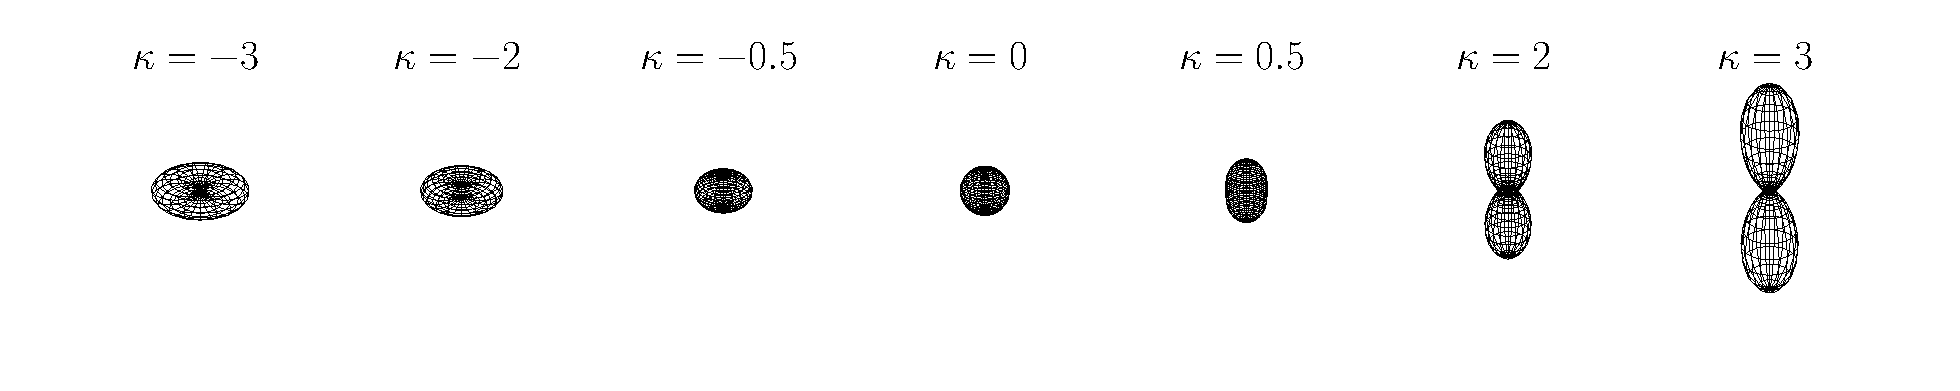
\includegraphics[width=1.0\textwidth, interpolate=true]{figs/watson.pdf}\\
\end{center}
\begin{align*}
  &f(\mh{r}; \bs{\hat{\mu}}, \kappa) = \frac{1}{4\pi{}_1F_1\left(\frac{1}{2}, \frac{3}{2}, \kappa\right)}\text{exp}\{\kappa (\bs{\hat{\mu}}^T\mh{r})^2\}\\
  &r \in \mathbb{RP}^2, \hat{\mu} \in \mathbb{RP}^2, \kappa \in \mathbb{R}
\end{align*}
\begin{itemize}
\item Expensive special function ${}_1F_1$
\item Can't take integrals or derivatives wrt $\kappa$
\item Can't take intensity integrals wrt $\hat{\mu}$
\end{itemize}
\end{frame}

\begin{frame}[label=sec-3]{Central Angular Gaussian Distribution}
\begin{align*}
  &f(\mh{r}; \mathbf{A}) = \frac{r^T\mathbf{A}r}{|\mathbf{A}|}\\
  &r \in \mathbb{RP}^2\\
  &\mathbf{A}\ \text{is a}\ 3\times 3\ \text{positive definite matrix}
\end{align*}
\begin{itemize}
\item Projection of a Gaussian in $\mathbb{R}^3$ into $\mathbb{RP}^2$
\item $\mathbf{A}$ defines a ellipsoid.
\item Too general for us. We want rotational symmetry. 
\end{itemize}
\end{frame}
\begin{frame}[label=sec-4]{Spheroid Distribution}
\vspace{-1em}
\begin{center}
  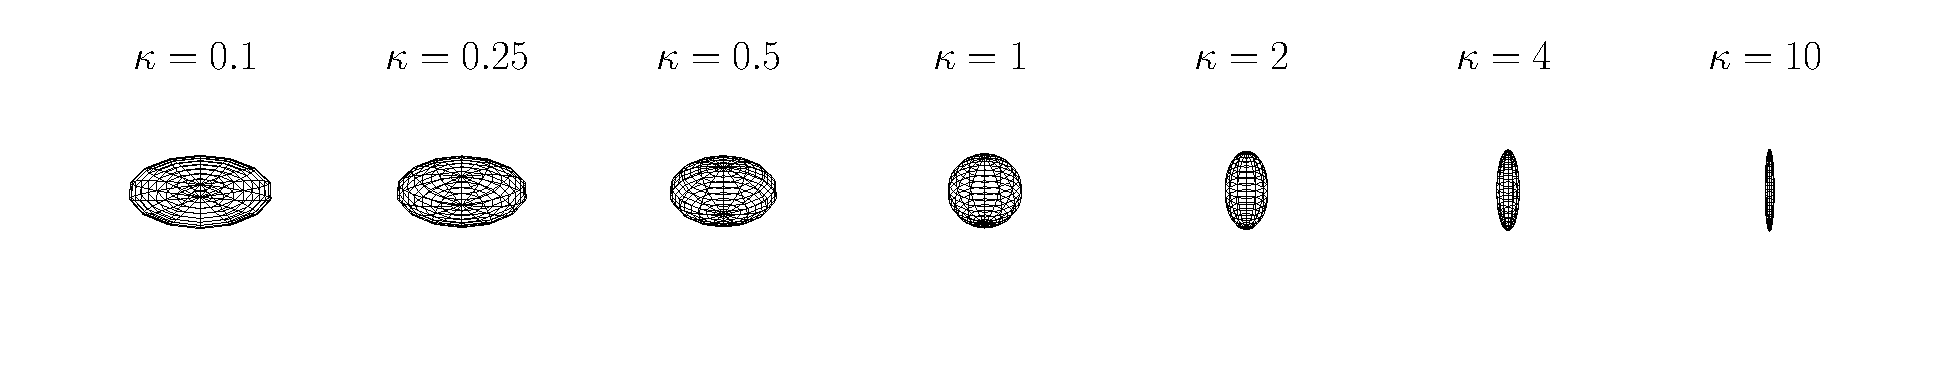
\includegraphics[width=1.0\textwidth, interpolate=true]{figs/spheroid.pdf}
\end{center}
\vspace{-4em}
\begin{align*}
  f(\mh{r}; \mathbf{A}) = \frac{r^T\mathbf{A}r}{|\mathbf{A}|}
\end{align*}
\vspace{-1em}
\begin{itemize}
\item $\mathbf{A}$ is a 3 $\times$ 3 positive definite matrix with 3 orthonormal evecs.
\item The first evec is pointed along the symmetry axis $\hat{\mu} \in \mathbb{RP}^2$
\item The other two evecs are have the same eigenvalue. 
\item The ratio of the symmetry evalue to orthogonal evalues is $\kappa^2$. 
\item Cheap to compute. Can take derivatives and integrals.
\item $\kappa$ has an easy interpretation---ratio of symmetry axis radius to orthogonal axis radius
\item Matches Rudolf's previous work with birefringent materials. We're comfortable reasoning about spheroids. 
\end{itemize}
\end{frame}

\begin{frame}[label=sec-5]{Next Topic: Optimization Problem}
\begin{align*}
f&: \mathbb{S}^2 \rightarrow \mathbb{R}\\ \\
x^* &= \underset{x\in \mathbb{S}^2}{\mathrm{argmin}}\ f(x)
\end{align*}
\begin{itemize}
\item What is the gradient of $f$?\\
\item Use spherical coordinates ($\theta$, $\phi$). $\nabla f \stackrel{?}{=} \left(\frac{\partial f}{\partial \theta}, \frac{\partial f}{\partial \phi})$
\item Step size is different at different points on the sphere.
\item Gradient depends on the coordinate choice. 
\item Trouble at the poles!
\end{itemize}
\end{frame}
\begin{frame}[label=sec-6]{Instead optimize on a manifold}
\begin{center}
  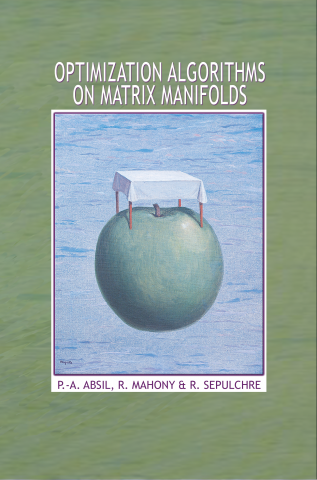
\includegraphics[width=0.4\textwidth, interpolate=true]{figs/book.png}\\
\end{center}
\end{frame}
\begin{frame}[label=sec-7]{Rough Recipe For Optimizing On A Manifold}
\begin{enumerate}
\item Let $f:\mathbb{S}^2 \rightarrow \mathbb{R}$ be the function we want to optimize. 
\item {Embed the manifold in Euclidean space and define a new smooth function $\bar{f}: \mathbb{R}^3 \rightarrow \mathbb{R}$. If we 
constrain $\bar{f}$ to $\mathbb{S}^2$ then we recover $f$.}
\item Choose an initial guess on $\mathbb{S}^2$. 
\item Take the usual Euclidean gradient of $\bar{f}$. $\nabla \bar{f} = \left(\frac{\partial f}{\partial x}, \frac{\partial f}{\partial y}, \frac{\partial f}{\partial z})$
\item Project the Euclidean gradient onto the tangent space of $\mathbb{S}^2$. This projected gradient is called the \textit{Riemannian gradient}. 
\item Update your guess by moving along the Riemannian gradient. 
\item \textit{Retract} your new guess from the tangent space back onto $\mathbb{S}^2$. 
\item Repeat from step 4.
\end{enumerate}
\end{frame}
\begin{frame}[label=sec-8]{}
\begin{center}
  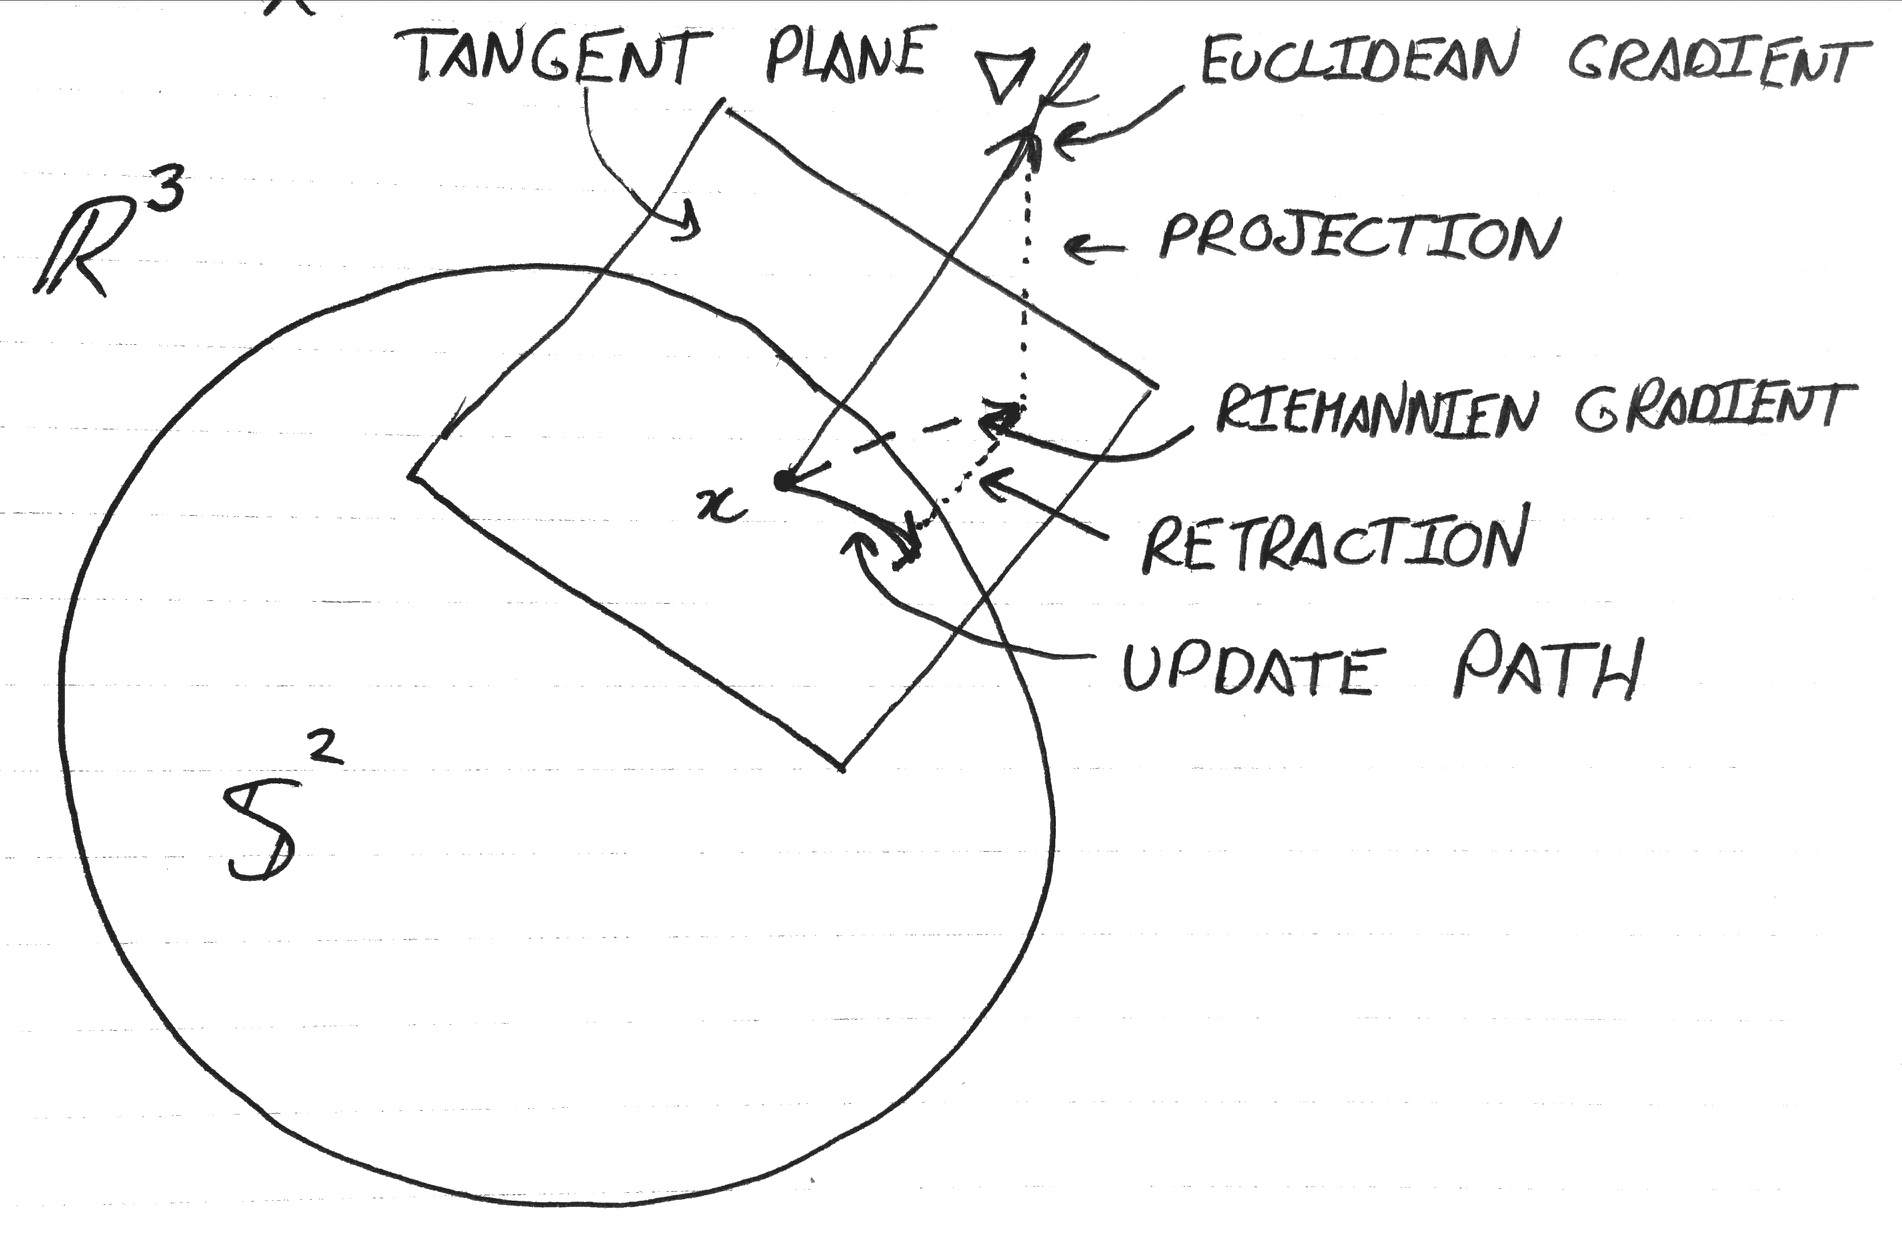
\includegraphics[width=1.0\textwidth, interpolate=true]{figs/tangent.pdf}\\
\end{center}
\end{frame}
\begin{frame}[label=sec-9]{Summary + Work In Progress}
\begin{itemize}
\item A central angular Gaussian distribution with rotational symmetry gives the spheroid distribution.
\item Spheroid distributions are easier to handle than Watson distributions.
\item I'm working on integrating the spheroid distribution analytically which will yield a much faster forward model.
\item Optimizing on an embedded manifold allows us to calculate gradients correctly.
\item Multiple seed gradient methods will be much faster than the gradient-free particle swarm methods I've been using.
\item Initial seed could be generated with Rudolf's proposed change of coordinates.
\end{itemize}
\end{frame}
% Emacs 25.3.1 (Org mode 8.2.10)
\end{document}